\documentclass[a4paper, 12pt]{article}
\usepackage[T1]{fontenc}
\usepackage[utf8]{inputenc}
\usepackage[english, italian]{babel}
\usepackage{amsmath,amssymb}
\usepackage{url}
\usepackage{graphicx}

\title{\bf Caratteristiche principali del modello NoSQL \textit{key-value}}
\author{Simone Richetti, mat. 129180, attività 3}
\date{}

\begin{document}

\maketitle

% Abstract
\begingroup\selectlanguage{english}
\begin{abstract}
Con l'esplosione dei \textit{Big Data}, diverse tipologie di applicazioni necessitano di performance e scalabilità più alte di quanto i tradizionali database relazionali potessero garantire. In questo contesto si sono sviluppati i database \textit{key-value}. Questi modelli sono caratterizzati dalla semplicità nella gestione e nell'accesso dei dati, la quale garantisce velocità nelle operazioni su essi, dalla scalabilità del sistema, la quale permette di ampliarlo con minimo impatto, e dall'alta disponibilità dei dati anche in condizioni critiche dei sistemi, necessaria per tutte quelle applicazioni in cui è importante la \textit{user experience} dei fruitori. Queste caratteristiche sono ottenute al prezzo di limiti su dimensioni e tipologie di dati trattabili e sulle operazioni che si possono eseguire su essi, oltre che ad una complessa gestione della consistenza dei dati in caso di \textit{failures} della rete o dei sistemi.
\end{abstract}\endgroup

\section{Introduzione}
Per molti anni i database relazionali sono stati la principale soluzione utilizzata dalla maggior parte dei sistemi per il salvataggio persistente dei dati e per la loro gestione.

Con la diffusione di servizi \textit{web-based} e le relativa gestione di grandi moli di dati, questo tipo di soluzioni ha iniziato ad evidenziare dei limiti strutturali. La difficoltà di questi sistemi a scalare con la quantità di dati in termini di performance nelle operazioni svolte hanno portato alla ricerca di soluzioni alternative per lo \textit{storage} dei dati.

In questo contesto si sono diffusi i primi database NoSQL e in particolare quelli di tipologia \textit{key-value}, che cercano di soddisfare questa richiesta di alte performance con la semplicità nell'accesso ai dati, un'alta scalabilità e con la distribuzione dei dati su diversi \textit{data storage}.

In questa relazione vengono approfondite le caratteristiche principali di questo modello NoSQL, facendo riferimento ad alcune sue implementazioni, in particolare a DynamoDB di Amazon. Dynamo è stato il primo tra i sistemi che implementano questo modello e ha introdotto le caratteristiche e le tecniche che sono state poi riprese dalle successive implementazioni.

\section{Caratteristiche}
Approfondiamo ora le principali caratteristiche dei database che implementano il modello \textit{key-value}: ci si concentrerà principalmente sulla rappresentazione e gestione dei dati e sulle tecniche utilizzate per garantire scalabilità e disponibilità dei dati, facendo riferimento alle caratteristiche di \textit{consistency}, \textit{availability} e \textit{partition-tolerance}.

\subsection{Gestione dei dati}
Mentre i database relazionali salvano i dati sotto forma di tabella con uno schema ben preciso, il modello \textit{key-value} salva i dati in una struttura simile ad un dizionario o ad una \textit{hash map}:
\begin{itemize}
    \item Il database è diviso in tabelle;
    \item Ogni tabella contiene una serie di \textit{record} o \textit{item}, che rappresentano i singoli oggetti;
    \item Ogni \textit{record} è definito come un'insieme di \textit{field}, ovvero coppie chiave-valore;
    \item Ogni \textit{record} è identificato univocamente da una \textit{partition key} che viene utilizzata per accedere a quell'elemento, ma anche per determinare in quale partizione esso verrà salvato, basandosi sul valore dell'\textit{hash} della chiave.
\end{itemize}

\begin{figure}[!ht]
    \centering
    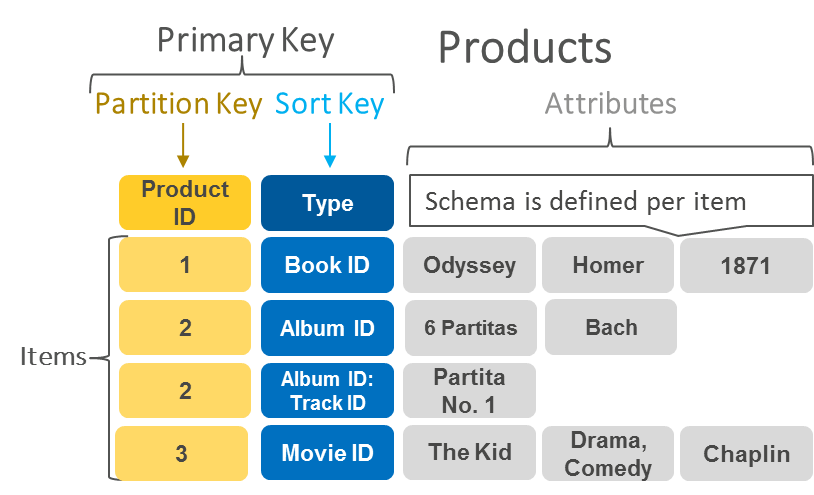
\includegraphics[width=.8\textwidth]{images/chiavevalore.png}
    \caption{Struttura chiave-valore dei dati}
    \label{fig:keyval}
\end{figure}

Nei sistemi più semplici, come ad esempio in Aerospike, le chiavi sono stringhe, mentre i valori sono salvati come \textit{blob}, ovvero come vettori di byte senza uno specifico tipo associato. Ci sono poi sistemi che invece supportano una tipizzazione dei dati, chi più semplice e chi invece, come ad esempio DynamoDB, permettendo anche strutture dati più complesse come dati geografici, collezioni di oggetti o campi innestati.

Molti sistemi che implementano il modello chiave-valore fanno utilizzo anche di una chiave aggiuntiva, detta \textit{sort key}, la quale viene utilizzata per ordinare i \textit{record} all'interno della partizione.

È importante notare come, fatta eccezione per la \textit{partition key} ed eventualmente la \textit{sorting key}, non esista uno schema fisso per i \textit{record}. Ogni oggetto ha uno schema a sé stante, ovvero diversi oggetti possono presentare diversi campi. Questo permette un grande risparmio di memoria, poiché non si devono salvare \textit{placeholder} o occupare memoria per campi che un oggetto non utilizza, al contrario di ciò che avviene nei database relazionali, e permette anche una minore complessità dal punto di vista della gestione dei dati e della velocità delle operazioni su di essi.

Questa flessibilità nello schema, però, rende limitato il numero ed il tipo di operazioni che si possono svolgere su questi dati. Per maggiori dettagli riguardo a questo si veda la sezione \ref{ops}.

L'hardware utilizzato per lo \textit{storage} dei dati varia a seconda delle necessità: sistemi come DynamoDB che hanno bisogno di persistenza utilizzano \textit{data storage} distribuiti basati su Dischi a Stato Solido (SSD), mentre ci sono altri sistemi chiamati \textit{in-memory}, come Memcached o Redis, che utilizzano principalmente la memoria DRAM per un accesso ad altissime prestazioni ai dati ed effettuano un salvataggio asincrono e periodico dei dati su dischi persistenti. L'utilizzo di una memoria volatile, però, genera il rischio di una perdita di dati nel caso di guasti e \textit{failures} del sistema o della rete, quindi è una soluzione utilizzata solo in sistemi in cui questa perdita è un rischio tollerabile. 

\subsection{Operazioni sui dati}\label{ops}
% Per garantire basse latenze nell'accesso ai dati, quest'ultimo è estremamente semplice per risultare molto veloce. D'altra parte, il meccanismo di lettura e scrittura di dati è estremamente limitato se comparato alle \textit{queries} SQL.

In generale, i database chiave-valore non hanno un linguaggio di \textit{query}, ma utilizzano delle semplici primitive per leggere e scrivere i dati: le funzioni \verb|get(key)| e \verb|put(key, object)|. La \verb|get| permette di ottenere un intero oggetto indicando la chiave che lo identifica, la \verb|put| permette di aggiungere e/o aggiornare un record. Alcuni database prevedono anche una primitiva aggiuntiva \verb|delete(key)| per rimuovere un oggetto, identificandolo con la sua chiave.

Da un lato, è proprio la semplicità di questo modello che rende i database \textit{key-value} veloci, scalabili, flessibili e semplici da utilizzare. I \textit{record} sono acceduti interamente con una richiesta diretta alla memoria. Non ci sono operazioni che riguardano molteplici oggetti, non c'è uno schema da cui recuperare dati, non c'è un \textit{query language} da tradurre.

D'altra parte, la semplicità del modello limita fortemente le tipologie di applicazioni che possono sfruttarlo. Un database di questo tipo permette solo l'accesso a singoli oggetti mediante la loro chiave: non ci sono \textit{join}, aggregazioni o proiezioni come in un database relazionale. Se si vogliono implementare operazioni di \textit{filtering} o di costruzione di una determinata \textit{view} sui dati, questo deve essere fatto a livello applicativo, aggiungendo un \textit{overhead} computazionale alle prestazioni del sistema.
% Si potrebbe dire che è proprio per questo che alcuni db NoSQL usano il modello chiave valore per salvare i dati ma poi lo estendono per fornire più operazioni, come ad esempio quelli a grafo. Bisogna però fare ricerche su questo.

%======================================================================


\subsection{\textit{High-availability} e scalabilità}
Per il tipo di servizi che devono supportare, i sistemi che implementano un modello \textit{key-value} devono garantire le seguenti caratteristiche chiave:
\begin{itemize}
    \item Scalabilità, per poter permettere una continua crescita;
    \item \textit{High-availability}, ovvero le operazioni di \textit{read} e \textit{write} devono andare sempre a buon fine;
    \item Resistenza a fallimenti senza impattare \textit{availability} e performance.
\end{itemize}

In sistemi i cui dati sono distribuiti su più nodi, il \textit{CAP theorem} evidenza come in condizioni critiche non sia possibile garantire contemporaneamente una forte consistenza dei dati e la loro immediata disponibilità. Molti sistemi tradizionali sacrificano la disponibilità dei dati per la loro consistenza, ad esempio non fornendo la risposa ad una richiesta fino a quando non si è certi della sua correttezza. Al contrario, il modello chiave-valore ha come target sistemi che prediligono scalabilità e disponibilità dei dati, sacrificando la consistenza sotto alcuni scenari di fallimento, ovvero sistemi in cui è fondamentale fornire una risposta ad ogni richiesta, a costo del fornire una risposta che non è garantita essere la più aggiornata e corretta possibile.

Oltre a queste caratteristiche fondamentali, possiamo trovare implementati in questi sistemi i seguenti principi chiave:

\begin{description}
\item [Simmetria] ogni nodo ha le stesse responsabilità degli altri, il sistema è distribuito senza nodi centrali con funzioni di comando o controllo;
\item [Decentralizzazione] estensione della simmetria, il design del sistema deve favorire tecniche di comunicazione di tipo \textit{peer-to-peer} piuttosto che uno schema di comando centralizzato. Questo permette di avere un sistema più scalabile e non crea \textit{single points of failure};
\item [Eterogeneità] il sistema deve sfruttare l'eterogeneità della struttura sottostante, ad esempio bilanciare il \textit{workload} sui singoli nodi in base alle capacità del singolo hardware.
\end{description}

Vediamo ora alcuni soluzioni di design che garantiscono le caratteristiche di scalabilità e disponibilità dei dati. I dettagli di design riportati nelle sezioni seguenti si riferiscono ad Amazon DynamoDB: potrebbero esserci quindi altri database che differiscono in tecniche utilizzate o caratteristiche implementate, si può però affermare che i principi che stanno alla base di esse accomunano la grande maggioranza dei sistemi che implementano un modello \textit{key-value}.


\subsubsection{\textit{Partitioning}: scalabilità}\label{part}
% Key-value stores scale out by implementing partitioning (storing data on more than one node), replication and auto recovery. They can scale up by maintaining the database in RAM and minimize the effects of ACID guarantees (a guarantee that committed transactions persist somewhere) by avoiding locks, latches and low-overhead server calls.
I database chiave-valore implementano soluzioni di \textit{partitioning} per assicurarsi scalabilità. I dati sono salvati in diversi nodi: questo permette di aggiungere e rimuovere facilmente nodi alla rete senza impattare l'intero sistema. Per nodo intendiamo ogni singola unità di \textit{storage} dei dati.

La distribuzione dei dati su diversi nodi si basa sull'\textit{hash} della \textit{primary key} di ogni record. Possiamo rappresentare l'architettura sottostante come un \textit{ring} di nodi, ad ogni nodo è associato un valore casuale che rappresenta la sua posizione nell'anello e quel nodo è responsabile di tutte le posizioni che vanno dalla posizione del suo predecessore alla sua posizione. La funzione di \textit{hashing} è creata in modo che il suo codominio equivalga allo spazio dei valori delle posizioni dei nodi, perciò il valore dell'\textit{hash} della \textit{primary key} di un \textit{record} indica quale nodo sia "responsabile" di esso. Questo nodo è chiamato \textit{coordinator node}.

\begin{figure}[!ht]
    \centering
    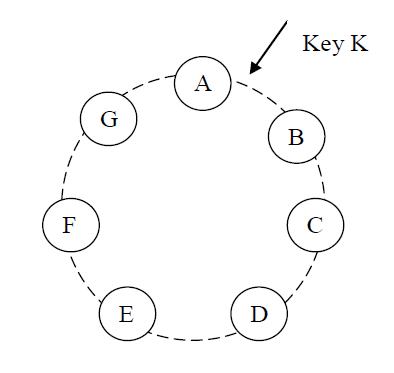
\includegraphics[width=.4\textwidth]{images/nodering.png}
    \caption{Data partitioning}
    \label{fig:part}
\end{figure}

Il vantaggio principale di questa tecnica, detta \textit{consistent hashing}, è dato dal fatto che l'aggiunta o la rimozione di un nodo impatta solo i nodi circostanti e non l'intero sistema, rendendo facile modificare la dimensione della rete di nodi, risultando in un sistema molto scalabile.

% Eventuale parlare di nodi virtuali per load balancing
%the basic
% algorithm is oblivious to the heterogeneity in the performance of
% nodes. To address these issues, Dynamo uses a variant of
% consistent hashing: instead of
% mapping a node to a single point in the circle, each node gets
% assigned to multiple points in the ring. To this end, Dynamo uses
% the concept of “virtual nodes”. A virtual node looks like a single
% node in the system, but each node can be responsible for more
% than one virtual node. Effectively, when a new node is added to
% the system, it is assigned multiple positions (henceforth, “tokens”)
% in the ring. The process of fine-tuning Dynamo’s partitioning
% scheme is discussed in Section 6.
% Using virtual nodes has the following advantages:
% • If a node becomes unavailable (due to failures or routine
% maintenance), the load handled by this node is evenly
% dispersed across the remaining available nodes.
% • When a node becomes available again, or a new node is
% added to the system, the newly available node accepts a
% roughly equivalent amount of load from each of the other
% available nodes.
% • The number of virtual nodes that a node is responsible can
% decided based on its capacity, accounting for heterogeneity
% in the physical infrastructure.

\subsubsection{\textit{Data replication}: \textit{availability}}
Per ottenere un'alta \textit{availability}, i sistemi chiave-valore replicano i dati su molteplici nodi: ogni record è affidato ad un \textit{coordinator node} che lo salva nel proprio storage e che si occupa di salvarne una copia sugli $N$ nodi successivi del \textit{ring}. La lista di nodi che contiene una determinata chiave è chiamata \textit{preference list}.

\begin{figure}[!ht]
    \centering
    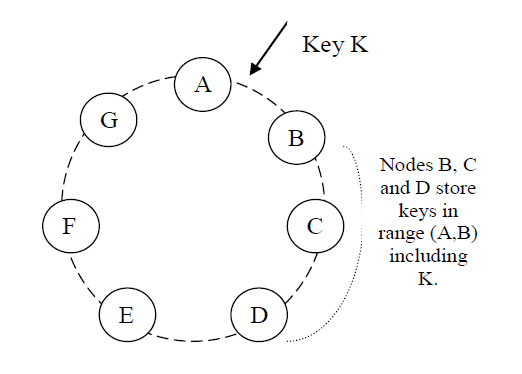
\includegraphics[width=.6\textwidth]{images/ringreplication.png}
    \caption{Data replication}
    \label{fig:rep}
\end{figure}

Il vantaggio della \textit{data replication} è una maggiore resistenza ai fallimenti della rete o dei singoli sistemi: se un nodo è irraggiungibile, posso recuperare i dati salvati su di esso da altri nodi. D'altra parte però, questo crea un problema dal punto di vista della consistenza: in certi istanti alcuni nodi che mantengono queste copie potrebbero essere irraggiungibili da eventuali aggiornamenti, rischiando così di avere delle copie conflittuali dello stesso dato. Un modo per gestire questi conflitti può essere l'utilizzo di \textit{data versioning}.

\subsubsection{\textit{Data versioning}: consistenza}
Abbiamo visto come, seguendo le logiche descritte dal \textit{CAP theorem}, i sistemi \textit{key-value} prioritizzino assolutamente disponibilità e scalabilità, accettando in situazioni critiche problemi di consistenza tra le diverse copie dei dati. Vediamo quindi come viene gestita la consistenza dei dati in situazioni ordinarie e come invece viene gestita la presenza di copie conflittuali dello stesso dato.

Database come DynamoDB e Cassandra garantiscono una \textit{eventual consistency}: in condizioni operative normali, le modifiche ad una copia sono propagate in maniera asincrona a tutte le repliche entro un certo lasso di tempo. Tuttavia, in condizioni di sovraccarico o guasti nella rete, le modifiche potrebbero non raggiungere tutte le copie per un tempo prolungato, generando la presenza di copie diverse di uno stesso dato per tutto il lasso di tempo.

Per gestire questa situazione, ogni modifica di un oggetto viene trattata come una sua nuova \textit{versione} e il sistema consente la convivenza di diverse versioni di uno stesso oggetto al suo interno. In condizioni normali, il sistema è in grado di riconoscere una versione come aggiornamento della precedente e quindi di portare tutte le copie alla versione più recente, ma in caso di \textit{failures} della rete combinate con modifiche concorrenti dello stesso oggetto potrebbero crearsi diverse versioni con \textit{histories} di modifiche diverse e non conciliabili tra loro. In questo caso, il sistema non può risolvere il conflitto e, in caso di \textit{read} sul dato, ritorna tutte le versioni differenti al client in modo che questo performi il \textit{merging} dei diversi \textit{branch} di modifiche in uno unico.


\begin{figure}[!ht]
    \centering
    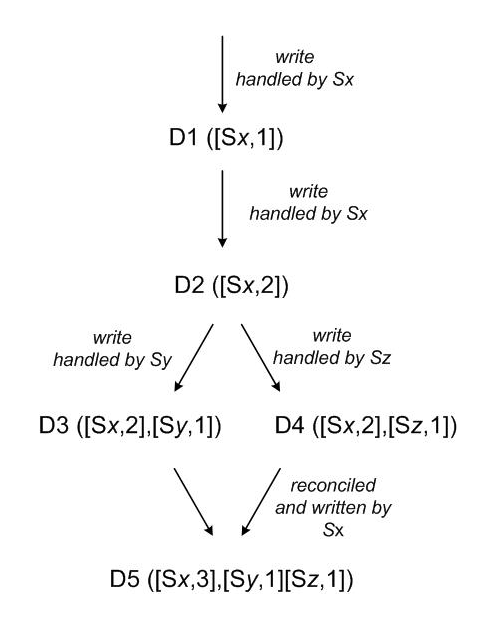
\includegraphics[width=.5\textwidth]{images/vectorclock.png}
    \caption{Evoluzione della versione e del vector clock di un oggetto}
    \label{fig:vecclock}
\end{figure}

Per gestire la risoluzione di conflitti di versione, DynamoDB utilizza la tecnica dei \textit{vector clocks}. Un \textit{vector clock} è una lista di coppie $(nodo, contatore)$: ad ogni versione di un oggetto è associato un \textit{vector clock} che contiene quali nodi hanno modificato quel record e quante volte. Quando un \textit{vector clock} è incluso in un altro, ovvero è stato modificato dagli stessi nodi con tutti i contatori minori o uguali a quelli dell'altro, si può supporre che il secondo sia la versione più aggiornata del primo e di conseguenza si aggiornano le copie che riportano una versione precedente. Altrimenti, se i due \textit{vector clocks} non sono associabili con nessun rapporto di parentela, allora le copie sono in conflitto: se il client effettua una \textit{read} in presenza di copie conflittuali, Dynamo ritorna tutte le copie presenti con relative versioni e \textit{clocks}. Un successivo \textit{update} di quel \textit{record} da parte del client viene visto come una riconciliazione del conflitto e tutte le copie vengono collassate nell'unica nuova versione dell'oggetto.

\section{Conclusioni}
Il punto di forza dei database \textit{key-value} risiede nelle loro alte performance dovute alla loro semplicità. L'accesso in memoria è diretto, senza un \textit{query language} e senza ottimizzazioni o \textit{filtering} dei dati, e i dati possono essere distribuiti su più storage con un design resistente a eventuali guasti della rete, risultando in un'immediata disponibilità dei dati e in un sistema scalabile. Queste caratteristiche rendono il modello chiave-valore ideale per sistemi \textit{always-on}, con forti requisiti di performance e che devono gestire grandi moli di dati. Per questo motivo, i database \textit{key-value} sono ampiamente utilizzati in casi d'uso come la memorizzazione di sessioni utente in applicazioni web, la gestione del carrello in grandi sistemi \textit{e-commerce} tra cui Amazon, gestione di profili utente e delle loro preferenze o sistemi di \textit{recommendation} di prodotti.

% For most key-value stores, the secret to its speed lies in its simplicity. The path to retrieve data is a direct request to the object in memory or on disk. The relationship between data does not have to be calculated by a query language; there is no optimization performed. They can exist on distributed systems and don’t need to worry about where to store indexes, how much data exists on each system or the speed of a network within a distributed system they just work.

% Some key-value stores like Aerospike, take advantage of other attributes to extend performance, such as using SSD’s or flash storage and implementing secondary indexes to continue to push the limits of today’s technology to places we’ve not yet conceived.

% %=====

% Generally speaking, the secret to key-value databases lies in their simplicity and the resulting speed that becomes available. Retrieving data requires a direct request (key) for the object in memory (value), and there is no query language. The data can be stored on distributed systems with no worries about where indexes are located, the volume of data, or network slowdowns. Some key-value databases are using flash storage and secondary indexes in an effort to push the limits of key-value technology.

% A key-value database is both easy to build and to scale. It typically offers excellent performance and can be optimized to fit an organization’s needs. When a key-value database is modified with new applications, there is an increased chance the system will operate more slowly.


\begin{thebibliography}{}
\bibitem[1]{dynamopaper} DeCandia G., Hastorun D., Jampani M., Kakulapati G., Lakshman A., Pilchin A., Sivasubramanian S., Vosshal P., Vogels W.; \textit{Dynamo: Amazon’s highly available key-value store.}; ACM SIGOPS symposium on Operating systems principles (2007), ACM Press New York, NY, USA, pp. 205–220.

\bibitem[2]{consistency} Si Liu, Nguyen S., Ganhotra J., Rahman M. R.,
Gupta I., Meseguer J., \textit{Quantitative Analysis of Consistency
in NoSQL Key-value Stores}, al link \url{https://assured-cloud-computing.illinois.edu/files/2014/03/Quantitative-Analysis-of-Consistency-in-NoSQL-Key-values-Stores-1.pdf}

\bibitem[3]{amazonkeyval} Pagina AWS su db \textit{key-value}:\\ \url{https://aws.amazon.com/it/nosql/key-value/}

\bibitem[4]{mediumarticle} Articolo su Medium sul confrontro tra RDB e \textit{key-value}:\\ \url{https://medium.com/@wishmithasmendis/from-rdbms-to-key-value-store-data-modeling-techniques-a2874906bc46}

\bibitem[5]{aerospikeintro} Introduzione di Aerospike ai db chiave-valore: \url{https://www.aerospike.com/what-is-a-key-value-store/}

\bibitem[6]{keyvalwiki} Pagina Wikipedia sul modello \textit{key-value}:\\ \url{https://en.wikipedia.org/wiki/Key-value_database}

\bibitem[7]{redisintro} Introduzione a Redis: \url{https://redis.io/topics/introductions}

\end{thebibliography}

\end{document}
